\section{Теория}

\subsection{Первый метод: нахождение argmax(Tol)}
Поскольку показания датчиков обладают погрешностью, полученные данные на самом деле следует рассматривать как интервалы, центр которых совпадает с измеренными показаниями, а радиус $\epsilon$ (в данном случае $\frac{1}{2^{14}} = \frac{1}{16384}$). 

Так как показания независимы, можно рассмотреть произвольную ячейку из всех $8 \times 1024$ ячеек. Тогда, для данной ячейки имеем $100 \times 11$ пар значений $(x, y)$, где $x$ -- координата соответствующая поданному напряжению и лежит в границах $[-0.5, 0.5]$, а $y$ координата представляет собой интервал с $wid = 2/16384$. Для того, чтобы найти точечную оценку коэффициентов калибровки, можно воспользоваться распознающим функционалом Tol. 

\begin{equation}
    \text{Tol}(x) = \text{Tol}(x, A, b) = \min_{1 \leq i \leq m} \left\{ \text{rad}\:b_i - \left| \text{mid}\:b_i - \sum_{j=1}^{n}a_{ij} x_j \right| \right\}.
\end{equation}

Где $A$ -- матрица:

\begin{equation}
    \begin{pmatrix}
        x_0 & 1 \\
        \vdots & \vdots \\
        x_m & 1
    \end{pmatrix},
\end{equation}

$b$ -- интервальный вектор:

\begin{equation}
    \begin{pmatrix}
        [y_0 - \epsilon, y_0 + \epsilon] \\
        \vdots \\
        [y_m - \epsilon, y_m + \epsilon]
    \end{pmatrix}
\end{equation}

Особенностью данного функционала является то, что допусковое множество решений системы $Ax = b$ можно описать как

\begin{equation}
    \{x \in \mathbb{R}^n \:|\: \text{Tol}(x, A, b) \geq 0\}
\end{equation}

Если $\text{Tol}(\arg\max(\text{Tol}), A, b) \geq 0$, то система совместная и $\arg\max(\text{Tol})$ можно считать результатом регрессии (а значит это вектор содержащий $\beta_0, \beta_1$).

Однако часто система не является совместной. В таком случае следует рассмотреть множество $\text{Tol}_i$

\begin{equation}
    \text{Tol}_i(x, A, b) = \text{rad}(b_i) - \left| \text{mid}(b_i) - \sum_{j=1}^{n}a_{ij}x_j \right|, \quad 1 \leq i \leq m
\end{equation}

Если существует $i$ для которого $\text{Tol}_i < 0$, то $\text{Tol} < 0$. При этом, чтобы $\text{Tol}_i \geq 0$ достаточно подобрать достаточно большой $\text{rad}(b_i)$.

Таким образом, в случае отсутствия совместности, следует пройтись по строчкам матрицы и элементам $b$. Если для некоторых из них $\text{Tol}_i < 0$, то нужно ''расширить'' интервал в правой части, чтобы добиться $\text{Tol}_i = 0$. Тогда очевидно, что $\text{Tol}(\arg\max(\text{Tol}), A, b)$ будет равен 0, а $\arg\max(\text{Tol})$ будет вектором искомых коэффициентов калибровки. 

\subsection{Второй метод: нахождение оценки при помощи твинной арифметики}
У описанного выше метода есть два основных недостатка:

\begin{enumerate}
    \item ''Расширение'' интервалов в правой части системы приводит к сильной погрешности на практике, т.к. интервалы расширяются в обе стороны: как в сторону регрессионной прямой, так и от нее.
    \item Результатом данного метода является лишь точечная оценка.
\end{enumerate}

В качестве альтернативы, предлагается другой метод, основанный на использовании твинной арифметики.

В первом методе брались все пары $(x_i, [y_i - \epsilon, y_i + \epsilon])$ и работа велась со всеми интервалами. В данном методе предлагается разделить $y_i$ в группы по 100 измерений в зависимости от соответствующего $x_i$. Тогда для каждого различного $x_i$ для конкретного датчика получится набор значений по которому можно определить внутреннюю и внешнюю оценку, и для каждого $x_i$ постороить твин $[[\underline{y_{i}^{in}}, \overline{y_{i}^{in}}], [\underline{y_{i}^{ex}}, \overline{y_{i}^{ex}}]]$.

Затем снова построим распознающий функционал $\text{Tol}$, но теперь

\begin{equation}
    A =
    \begin{pmatrix}
        x_1 & 1\\
        x_1 & 1\\
        x_1 & 1\\
        x_1 & 1\\
        \vdots & \vdots\\
        x_n & 1
    \end{pmatrix}, \quad
    b =
    \begin{pmatrix}
        [\underline{y_{1}^{in}}, \overline{y_{1}^{in}}]\\
        [\underline{y_{1}^{ex}}, \overline{y_{1}^{in}}]\\
        [\underline{y_{1}^{in}}, \overline{y_{1}^{ex}}]\\
        [\underline{y_{1}^{ex}}, \overline{y_{1}^{ex}}]\\
        \vdots \\
        [\underline{y_{n}^{ex}}, \overline{y_{n}^{ex}}]
    \end{pmatrix}
\end{equation}

Если $\text{Tol}(\arg\max(\text{Tol})) = 0$, то так же возвращаем $\arg\max(\text{Tol})$. 

Если $\text{Tol}(\arg\max(\text{Tol})) > 0$, то можно найти множество значений $(\beta_0, \beta_1)$, при которых $\text{Tol} > 0$ и вернуть его.

Если $\text{Tol}(\arg\max(\text{Tol})) < 0$ снова требуется решить проблему отсутствия совместимости.

Для этого снова рассмотрим $\text{Tol}_i$, однако, вместо изменения правой части, будем убирать соответствующую строку из $A$ и $b$. В силу того что для каждой пары $(x_j, y_j)$ создается 4 уравнения, при удалении описанным способом несовместимых уравнений, уравнений останется больше, чем при первом способе. А значит решение будет точнее. При этом, в результате данной операции, возможна ситуация, когда $\text{Tol}(\arg\max(\text{Tol})) > 0$.

\subsection{Построение коридора совместимости}
\textbf{Определение:} Пусть в задаче восстановления зависимостей информационное множество $\Omega$ параметров зависимостей $y=f(x,\beta)$, совместных с данными, является непустым. Коридором совместных зависимостей рассматриваемой задачи называется многозначное отображение $\Gamma$, сопоставляющее каждому значению аргумента $x$ множество:

\begin{equation}
    \Gamma(x)=\bigcup_{\beta \in \Omega}f(x,\beta).
\end{equation}

В данном случае:

\begin{equation}
    f(x,\beta_0,\beta_1)=\beta_0x+\beta_1.
\end{equation}

Поэтому для построения коридора совместных зависимостей нужно для каждого отрезка $[x_i, x_{i+1}]$ найти нижнюю и верхнюю ограничивающую прямую из множества допустимых.

Для получения интересующих нас прямых рассматриваем вершины $\{v_0, ..., v_k\}$, где $v_p = (\beta_{p_0}, \beta_{p_1})$, выпуклого многоугольника - допускового множества решений. Для этого вычислим:

\begin{equation}
    \overline{p_i} = \arg\max_{1 \leq p \leq k}{\left\{ \beta_{p_0} \frac{x_i + x_{i+1}}{2} + \beta_{p_1} \right\}} 
    ;\quad 
    \underline{p_i} = \arg\min_{1 \leq p \leq k}{\left\{ \beta_{p_0} \frac{x_i + x_{i+1}}{2} + \beta_{p_1} \right\}}
\end{equation}

\noindent индексы верхней и нижней ограничивающих прямых на отрезке $[x_i, x_{i+1}]$.

\begin{figure}[H]
    \centering
    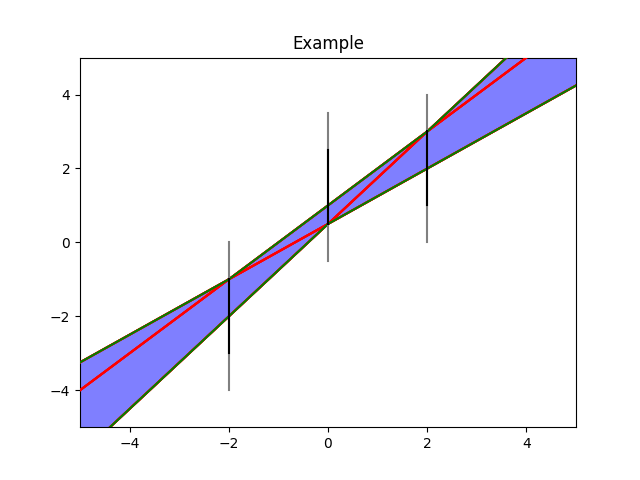
\includegraphics[width=0.8\linewidth]{image/example.png}
    \caption{Иллюстрация построения коридора совместности по вершинам множества допустимых значений. Твины обозначены серым и черным, прямые в вершинах -- красным, выбранные отрезки прямых -- зеленым.}
    \label{fig:chip}
\end{figure}

Рассмотрим этот пример подробнее.

Изначальные интервалы:

\begin{table}[H]
    \centering
    \begin{tabular}{|c|c|c|c|c|c|}
        \hline
        $i$ & $x$ & $\underline{y^{in}}$ & $\overline{y^{in}}$ & $\underline{y^{ex}}$ & $\overline{y^{ex}}$ \\ \hline
        0 & -2 & -3.0 & -1.0 & -4.0 & 0.0\\ \hline
        1 & 0 & 0.5 & 2.5 & -0.5 & 3.5\\ \hline
        2 & 2 & 1.0 & 3.0 & 0.0 & 4.0\\ \hline
    \end{tabular}
    \caption{Начальные данные}
    \label{tab:my_label}
\end{table}

Для допускового множества получаем следующие вершины:

\begin{table}[H]
    \centering
    \begin{tabular}{|c|c|}
        \hline
        $\beta_0$ & $\beta_1$ \\ \hline
        1.2510 & 0.4990 \\ \hline
        0.7490 & 0.4990 \\ \hline
        1.0000 & 1.0010 \\ \hline
    \end{tabular}
    \caption{Полученные вершины допускового множества}
    \label{tab:my_label}
\end{table}

Пусть $\text{value} = \arg\min_{1 \leq p \leq k}{\left\{ \beta_{p_0} \frac{x_i + x_{i+1}}{2} + \beta_{p_1} \right\}}$. Тогда для каждой границы интервала получим следующее (для интервала до и после последнего добавим дополнительные $x$: -5 и 5 соответственно. Фактически эти участки бесконечно ''длинные'').

\begin{table}[H]
    \centering
    \begin{tabular}{|c|c|c|c|}
        \hline
        $i$ & $\beta_0$ & $\beta_1$ & $\text{value}$ \\ \hline
        0 & 1.2510 & 0.4990 & -3.8794 \\ \hline
        1 & 0.7490 & 0.4990 & -2.1226 \\ \hline
        2 & 1.0 & 1.0010 & -2.4990 \\ \hline
    \end{tabular}
    \caption{Полученные значения для отрезка $[-5, -2]$}
    \label{tab:my_label}
\end{table}

Выбраны следующие индексы: $\underline{p_i}$ = 0, $\overline{p_i}$ = 1.

\begin{figure}[H]
    \centering
    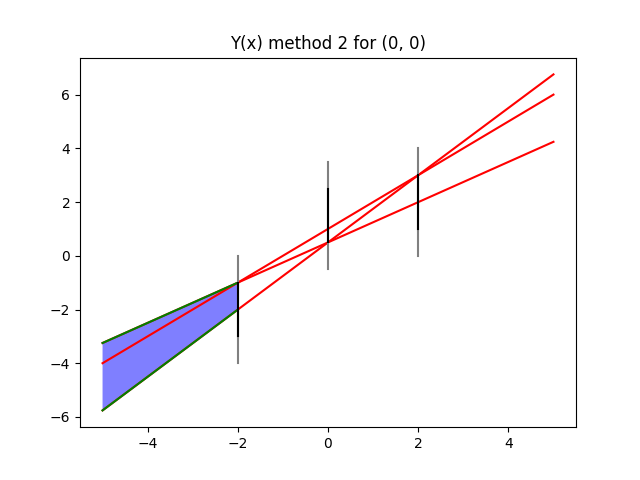
\includegraphics[width=0.8\linewidth]{image/0_example.png}
    \caption{Иллюстрация построения коридора совместности по вершинам множества допустимых значений на первом участке. Голубым обозначена часть коридора, красным ограничивающие прямые, зеленым границы построенной части коридора.}
    \label{fig:my_label}
\end{figure}

\begin{table}[H]
    \centering
    \begin{tabular}{|c|c|c|c|}
        \hline
        $i$ & $\beta_0$ & $\beta_1$ & $\text{value}$ \\ \hline
        0 & 1.2510 & 0.4990 & -0.7520 \\ \hline
        1 & 0.7490 & 0.4990 & -0.2500 \\ \hline
        2 & 1.0000 & 1.0010 & 0.0010 \\ \hline
    \end{tabular}
    \caption{Полученные значения для отрезка $[-2, 0]$}
    \label{tab:my_label}
\end{table}

Выбраны следующие индексы: $\underline{p_i}$ = 0, $\overline{p_i}$ = 2.

\begin{figure}[H]
    \centering
    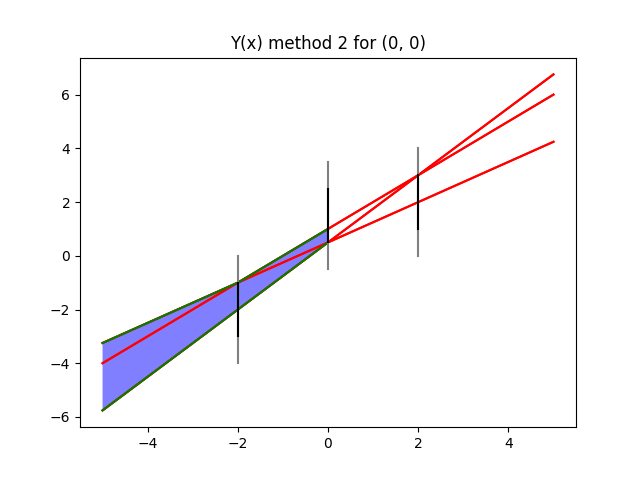
\includegraphics[width=0.8\linewidth]{image/1_example.png}
    \caption{Иллюстрация построения коридора совместности по вершинам множества допустимых значений на втором участке. Голубым обозначена часть коридора, красным ограничивающие прямые, зеленым границы построенной части коридора.}
    \label{fig:my_label}
\end{figure}

\begin{table}[H]
    \centering
    \begin{tabular}{|c|c|c|c|}
        \hline
        $i$ & $\beta_0$ & $\beta_1$ & $\text{value}$ \\ \hline
        0 & 1.2510 & 0.4990 & 1.7500 \\ \hline
        1 & 0.7490 & 0.4990 & -1.2480 \\ \hline
        2 & 1.0000 & 1.0010 & 2.0010 \\ \hline
    \end{tabular}
    \caption{Полученные значения для отрезка $[0, 2]$}
    \label{tab:my_label}
\end{table}

Выбраны следующие индексы: $\underline{p_i}$ = 1, $\overline{p_i}$ = 2.

\begin{figure}[H]
    \centering
    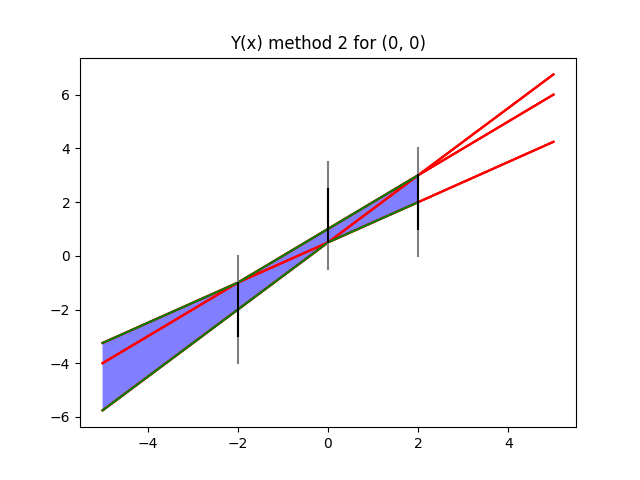
\includegraphics[width=0.8\linewidth]{image/2_example.png}
    \caption{Иллюстрация построения коридора совместности по вершинам множества допустимых значений на третьем участке. Голубым обозначена часть коридора, красным ограничивающие прямые, зеленым границы построенной части коридора.}
    \label{fig:my_label}
\end{figure}

\begin{table}[H]
    \centering
    \begin{tabular}{|c|c|c|c|}
        \hline
        $i$ & $\beta_0$ & $\beta_1$ & $\text{value}$ \\ \hline
        0 & 1.2510 & 0.4990 & 4.8744 \\ \hline
        1 & 0.7490 & 0.4990 & 3.1206 \\ \hline
        2 & 1.0000 & 1.0010 & 4.5010 \\ \hline
    \end{tabular}
    \caption{Полученные значения для отрезка $[2, 5]$}
    \label{tab:my_label}
\end{table}

Выбраны следующие индексы: $\underline{p_i}$ = 1, $\overline{p_i}$ = 0.

\begin{figure}[H]
    \centering
    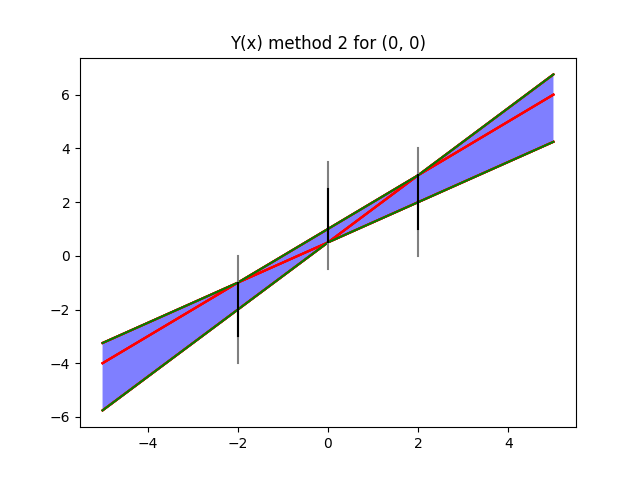
\includegraphics[width=0.8\linewidth]{image/3_example.png}
    \caption{Иллюстрация построения коридора совместности по вершинам множества допустимых значений на четвертом участке. Голубым обозначена часть коридора, красным ограничивающие прямые, зеленым границы построенной части коридора.}
    \label{fig:my_label}
\end{figure}